\documentclass[zihao=false,fontset=windows]{ctexart}
% ctexart 不接受任意 pt 选项。正文改 {10pt}，方括号里是行距。
\usepackage{scrextend}
\changefontsizes[12pt]{10pt}

\usepackage[a4paper,left=2.35cm,right=2.35cm,top=1.7cm,bottom=1.9cm]{geometry}
\usepackage{xcolor}
\usepackage{graphicx}
\usepackage{amsmath,amssymb}
\usepackage{enumitem}
\usepackage{tabularx}
\usepackage{colortbl}
\usepackage{listings}
\usepackage{hyperref}
\usepackage[most]{tcolorbox}

\definecolor{feishuText}{RGB}{31,35,41}
\definecolor{feishuBlue}{RGB}{36,91,219}
\definecolor{feishuRed}{RGB}{216,57,49}
\definecolor{feishuGray}{RGB}{100,106,115}
\definecolor{feishuGray2}{RGB}{143,149,158}
\definecolor{feishuPinkBg}{RGB}{251,191,188}
\definecolor{quoteBar}{RGB}{51,112,255}
\definecolor{codebg}{RGB}{245,246,247}
\definecolor{codeborder}{RGB}{222,224,227}
\definecolor{inlinebg}{RGB}{242,243,245}
\definecolor{callRed}{RGB}{253,226,226}
\definecolor{callOrange}{RGB}{255,245,235}
\definecolor{callYellow}{RGB}{254,255,240}
\definecolor{callGreen}{RGB}{240,251,239}
\definecolor{callBlue}{RGB}{240,244,255}
\definecolor{callRedSoft}{RGB}{254,241,241}
\definecolor{callSun}{RGB}{255,255,204}
\definecolor{tableHead}{RGB}{242,243,245}
\definecolor{tableRule}{RGB}{222,224,227}
\definecolor{codeText}{RGB}{31,35,41}
\definecolor{codeKeyword}{RGB}{0,0,255}
\definecolor{codeComment}{RGB}{0,128,0}
\definecolor{codeString}{RGB}{163,21,21}

\setmainfont{Times New Roman}
\setCJKmainfont{Microsoft YaHei}[AutoFakeBold=2.2]
\setCJKsansfont{Microsoft YaHei}[AutoFakeBold=2.2]
\setCJKmonofont{Microsoft YaHei}[AutoFakeBold=2.2]
\setmonofont{Consolas}
\newfontfamily\emojifont{Segoe UI Emoji}

\hypersetup{
  colorlinks=true,
  urlcolor=feishuBlue,
  linkcolor=feishuBlue,
  unicode=true,
  pdftitle={DeepSeek OCR}
}

\setlength{\parindent}{0pt}
\setlength{\parskip}{0.42em}
\setlength{\fboxsep}{1.5pt}
\setlength{\emergencystretch}{3em}
\linespread{1.28}
\color{feishuText}
\arrayrulecolor{tableRule}
\urlstyle{same}

\setlist[enumerate]{label=\textcolor{feishuBlue}{\arabic*.}, leftmargin=1.7em, itemsep=0.22em, topsep=0.28em, parsep=0.08em, partopsep=0pt}
\setlist[itemize,1]{label=\textcolor{feishuBlue}{\textbullet}, leftmargin=1.35em, itemsep=0.18em, topsep=0.25em, parsep=0.06em, partopsep=0pt}
\setlist[itemize,2]{label=\textcolor{feishuBlue}{◦}, leftmargin=1.45em, itemsep=0.12em, topsep=0.15em}
\setlist[itemize,3]{label=\textcolor{feishuBlue}{\rule[0.18em]{0.38em}{0.38em}}, leftmargin=1.55em, itemsep=0.1em, topsep=0.12em}

\newcommand{\feiEmoji}[1]{{\emojifont #1}}
\newcommand{\incode}[1]{\colorbox{inlinebg}{\ttfamily\small #1}}
\newcommand{\bigmath}[1]{%
  \begin{center}\large$\displaystyle #1$\end{center}%
}

\lstset{
  language=Python,
  basicstyle=\ttfamily\footnotesize\color{codeText},
  keywordstyle=\color{codeKeyword},
  commentstyle=\color{codeComment},
  stringstyle=\color{codeString},
  showstringspaces=false,
  breaklines=true,
  columns=fullflexible,
  keepspaces=true,
  tabsize=4,
  upquote=true,
  aboveskip=2pt,
  belowskip=0pt,
  xleftmargin=0pt,
  frame=none
}

\tcbset{
  feishubase/.style 2 args={
    enhanced,
    boxrule=0pt,
    arc=8pt,
    left=10pt,
    right=10pt,
    top=7pt,
    bottom=7pt,
    before skip=6pt,
    after skip=6pt,
    colback=#1,
    colframe=#1,
    before upper={\feiEmoji{#2}\hspace{0.45em}\ignorespaces}
  }
}
\newtcolorbox{feishubox}[2]{feishubase={#1}{#2}, breakable}
\newtcolorbox{feishuboxnb}[2]{feishubase={#1}{#2}}

\newtcolorbox{feishuquote}{
  enhanced,
  breakable,
  boxrule=0pt,
  leftrule=3pt,
  arc=0pt,
  colframe=quoteBar,
  colback=white,
  left=8pt,
  right=2pt,
  top=2pt,
  bottom=2pt,
  before skip=4pt,
  after skip=4pt,
  before upper=\color{feishuGray}
}

\newtcolorbox{feishucode}{
  enhanced,
  breakable,
  colback=codebg,
  colframe=codeborder,
  boxrule=0.6pt,
  arc=6pt,
  left=6pt,
  right=6pt,
  top=5pt,
  bottom=4pt,
  before skip=6pt,
  after skip=6pt
}


\usepackage{needspace}
\newcommand{\feihone}[2]{\par\vspace{1.15em}\Needspace{4\baselineskip}\noindent{\zihao{-2}\bfseries\textcolor{feishuBlue}{#1}\hspace{0.35em}#2}\par\vspace{0.28em}}
\newcommand{\feihtwo}[2]{\par\vspace{0.95em}\Needspace{4\baselineskip}\noindent{\zihao{3}\bfseries\textcolor{feishuBlue}{#1}\hspace{0.35em}#2}\par\vspace{0.28em}}
\begin{document}
{\zihao{1}\bfseries DeepSeek OCR\par}
% 来源：https://scnajei2ds6y.feishu.cn/wiki/LDyiwQuxWiyLT4kYBmVcnv89nwe
% 按用户要求省略3个代码块；知识文字和6幅非公式图保留。
% fig-16/19/23为浏览器pageAssets下载PNG；fig-28/30/73为正常页面截图裁切，73由两个重叠视口拼接。
\begin{feishubox}{callBlue}{☘}


论文：\href{https://github.com/deepseek-ai/DeepSeek-OCR/blob/main/DeepSeek_OCR_paper.pdf}{《DeepSeek-OCR: Contexts Optical Compression》}\par

模型仓库：\href{https://huggingface.co/deepseek-ai/DeepSeek-OCR}{deepseek-ai/DeepSeek-OCR}\par

代码仓库：\href{https://github.com/deepseek-ai}{deepseek-ai/DeepSeek-OCR}\par

\end{feishubox}

LLM 处理长文本时计算量正比于序列长度平方，因此面临效率问题。\textcolor{feishuRed}{\textbf{DeepSeek OCR 提出视觉模态可以作为文本信息的高效压缩媒介}}，将文本的图片作为 MLLM 的输入，并且利用视觉编码器压缩视觉 token 长度，实现单张包含文本的图像能以更少token表达丰富信息，达到比数字文本更高的压缩比。关键技术：\par

\textbf{DeepEncoder架构}：串连了SAM（local attention）+ Conv（压缩视觉序列长度）+ CLIP ViT（global attention）的视觉编码器，并且数据流宽度上，融合了 Local Feature 和 Global Feature 两路数据流\par

\textbf{\href{https://scnajei2ds6y.feishu.cn/wiki/HTJVw44IJibX6gkYWtlc1zCYnVh}{LLaVA-1.5(2023, Microsoft Research)}}\textbf{模式的动态分辨率}：不使用\href{https://scnajei2ds6y.feishu.cn/wiki/N6PmwVkCcisDJGkC7Ypc1SfInwh}{NaViT}的2D RopE动态分辨率方案，而是使用一个全图+多个Patch特征在\incode{seq\_len}上进行拼接从而捕捉全局和局部信息。\par

\feihone{1.}{模型架构}

模型结构图参考下官方图（左），看起来似乎和现在的三段式 MLLM 的结构不一样，其实本质是一样的，可以参考（右）图，模型还是可以划分为Visual Encoder、Projector、LLM三个部分，\textcolor{feishuRed}{只不过架构上最大的更改其实只有视觉编码器 }\textcolor{feishuRed}{\textbf{Deep Encoder 部分}}\textbf{：}\par

\begin{itemize}

\item 在结构深度上，串连了SAM（local attention）+ Conv（压缩视觉序列长度）+ CLIP ViT（global attention）

\item 在数据流宽度上，分别处理 Local Feature（Patch内） 和 Global Feature（Patch间）

\end{itemize}

\begin{tcbraster}[raster columns=2,raster equal height=rows,raster column skip=9pt,raster left skip=0pt,raster right skip=0pt]
\begin{tcolorbox}[blankest,width=\linewidth]
\begin{center}
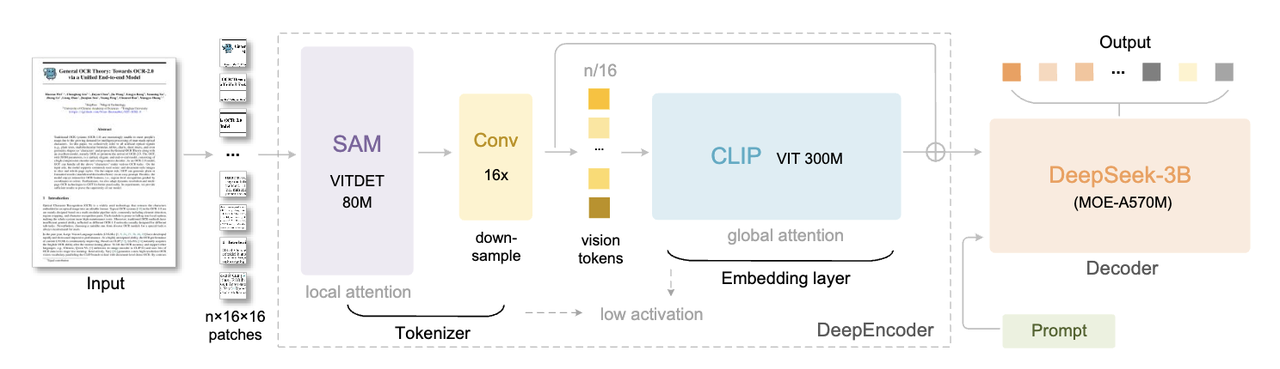
\includegraphics[width=\linewidth,height=0.80\textheight,keepaspectratio]{images/DeepSeek-OCR/fig-16.png}
\par {\small\color{feishuGray} 模型结构}
\end{center}
\end{tcolorbox}
\begin{tcolorbox}[blankest,width=\linewidth]
\begin{center}
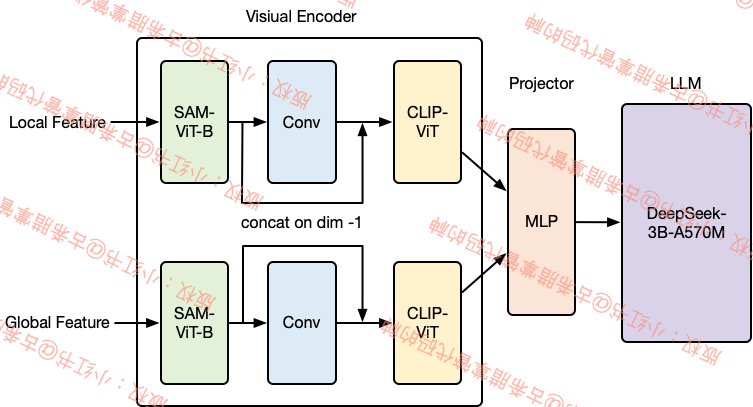
\includegraphics[width=\linewidth,height=0.80\textheight,keepaspectratio]{images/DeepSeek-OCR/fig-19.png}
\par {\small\color{feishuGray} 模型数据流}
\end{center}
\end{tcolorbox}
\end{tcbraster}

\feihtwo{1.1}{Deep Encoder }

Deep Encoder 由 SAM（local attention）+ Conv（压缩视觉序列长度）+ CLIP ViT（global attention）组成。\par

SAM首先用于最先提取特征，架构和\href{https://scnajei2ds6y.feishu.cn/wiki/B2SDwuImjimZ4TksKCpcF7e9nnb}{DeepSeek VL}中是类似的，需要注意的点就是在代码实现的时候 Conv（压缩视觉序列长度）的结构也被写在了 SAM 里：\par

\begin{center}
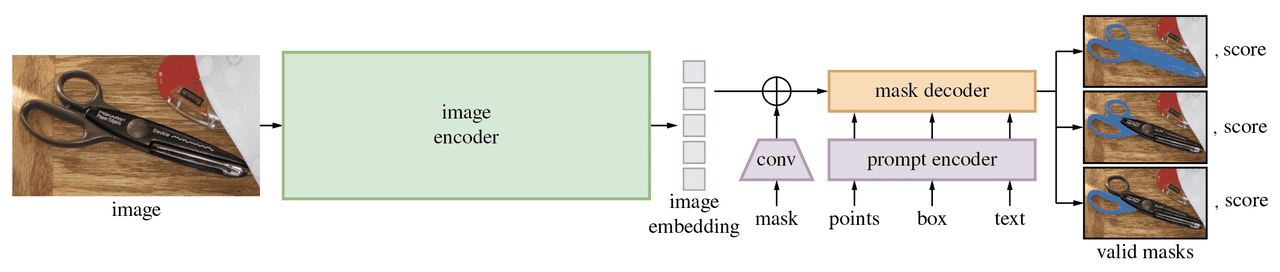
\includegraphics[width=0.98\linewidth,height=0.80\textheight,keepaspectratio]{images/DeepSeek-OCR/fig-23.png}

\end{center}

注意看在 SAM 结构里的 \textcolor{feishuRed}{\textbf{net\_2 }}和\textcolor{feishuRed}{\textbf{ net\_3 }}在 SAM 的输出侧就在\incode{seq\_len}完成了 4x4 = 16 倍的下采样，即压缩了视觉 token 长度：\par

% 原网页代码块 25 已按用户要求省略。

然后在 Conv 后就是一个标准的 ViT 结构用于提取特征，但是需要注意两个点：\par

\begin{itemize}

\item DeepSeek OCR 分别对 Local Feature（Patch内） 和 Global Feature（Patch间）进行特征提取，最后再 seq\_len 上进行拼接，这点和\href{https://scnajei2ds6y.feishu.cn/wiki/HTJVw44IJibX6gkYWtlc1zCYnVh}{LLaVA-1.5(2023, Microsoft Research)}实现高分辨率的方案类似，也就是\textcolor{feishuRed}{论文中支持动态分辨率的Gundam模型}：

\end{itemize}

\begin{center}
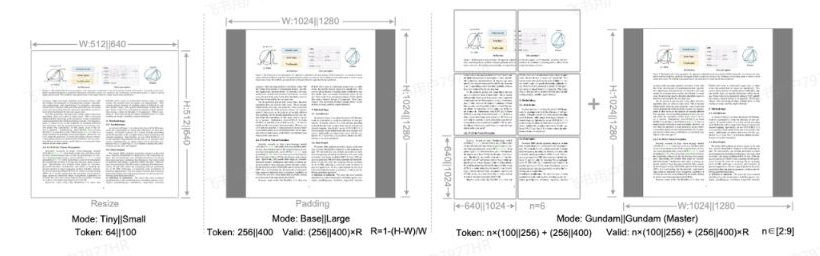
\includegraphics[width=0.98\linewidth,height=0.80\textheight,keepaspectratio]{images/DeepSeek-OCR/fig-28.png}

\end{center}

\begin{itemize}

\item 在 ViT 处理特征的时候，会同时处理 SAM 输出前后的特征，即类似一个 residual。

\end{itemize}

\begin{center}
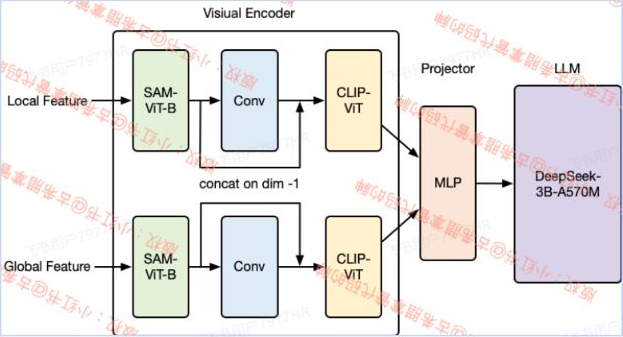
\includegraphics[width=0.98\linewidth,height=0.80\textheight,keepaspectratio]{images/DeepSeek-OCR/fig-30.png}
\par {\small\color{feishuGray} 模型数据流}
\end{center}

具体实现上参考代码：\par

% 原网页代码块 32 已按用户要求省略。

\feihtwo{1.2}{Projector}

Projector 的本质就是单层 Linear，这个和\href{https://scnajei2ds6y.feishu.cn/wiki/BNWJwSLQiizLZqkoQRtc4Pc5nPj}{LLaVA(2023, Microsoft)}是一样的，也可以参考\href{https://scnajei2ds6y.feishu.cn/wiki/KQDVwj7bAiSz8akJd3ecLLPank3?from=from_copylink}{MLLM 之 MLP Projector 发展史}：\par

% 原网页代码块 36 已按用户要求省略。

唯一的区别在于维度变化上，这是由于上一层结构\incode{DeepEncoder V2}的维度决定的：\par

\begin{itemize}

\item OCR-V1 \incode{2048 -> 1280}

\item OCR-V2 \incode{896 -> 1280}

\end{itemize}

\feihtwo{1.3}{LLM}

采用3B参数的MoE架构（DeepSeek3B-MoE），推理时激活6/64个专家，实际激活参数约570M。‘模型支持8192 token的超长序列处理，并且会进行文本数据（占总训练数据10\%）与多模态数据的混合训练。\par

\feihone{2.}{模型训练}

两阶段训练，说起来\textcolor{feishuRed}{\textbf{其实和其他通用 MLLM 比较类似，先对齐，再Instruction Tuning。}}\par

\feihtwo{2.1}{第一阶段：DeepEncoder 单独训练}

这里首先是替换了LLM部分，替换为一个Dense Model，然后\textcolor{feishuRed}{冻结LLM部分，只训练DeepEncoder}。\par

损失函数依然采用 next token prediction，使用OCR 1.0/2.0数据和100M LAION数据集采样数据，\par

\textbf{训练配置}\par

\begin{itemize}

\item 2个epoch训练周期

\item 1280批量大小

\item AdamW优化器

\item 5e-5初始学习率

\item cosine annealing学习率调度

\end{itemize}

\feihtwo{2.2}{第二阶段：DeepSeek-OCR 整体训练}

使用混合数据（70\% OCR数据/20\%通用视觉数据/10\%纯文本数据）进行分布式训练，猜测应该是全参数进行训练。\par

\textcolor{feishuRed}{\textbf{多分辨率拓展}}通过动态位置编码插值实现多模式联合训练：\par

\begin{itemize}

\item 原生分辨率模式：512×512(64 tokens)/640×640(100 tokens)/1024×1024(256 tokens)/1280×1280(400 tokens)

\item Gundam动态模式：局部640×640切片+全局1024×1024视图，支持超高清输入

\end{itemize}

\textbf{架构配置}\par

\begin{itemize}

\item 流水线并行（PP）分4段：PP0/PP1为DeepEncoder（冻结SAM-compressor参数，训练CLIP），PP2/PP3为MoE解码器

\item 3B MoE解码器激活570M参数，专家路由选择6/64激活专家+2共享专家

\end{itemize}

\textbf{训练参数}\par

\begin{itemize}

\item 20节点 8xA100-40G 集群

\item 40数据并行度，640全局批量

\item AdamW优化器，3e-5初始学习率

\item 文本数据训练速度90B tokens/天，多模态数据70B tokens/天

\end{itemize}

\feihone{3.}{实验}

可以看出小红书的\href{https://scnajei2ds6y.feishu.cn/wiki/AB2KwphPGiz6SCkIL27cNtT6nce}{dots.ocr}还是不错的，实测的效果也比 DeepSeek OCR要好。\par

\begin{center}
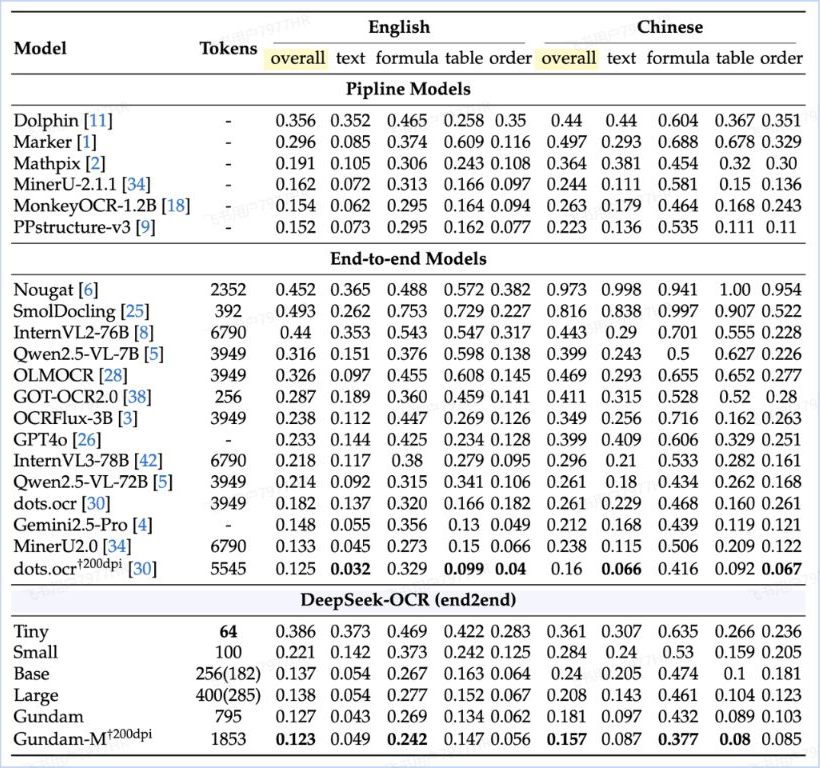
\includegraphics[width=0.98\linewidth,height=0.80\textheight,keepaspectratio]{images/DeepSeek-OCR/fig-73.png}

\end{center}

\end{document}